\documentclass[tikz,border=2pt,11pt]{standalone}
\usetikzlibrary{arrows.meta}
\usetikzlibrary{calc}
\usetikzlibrary{positioning}
\usepackage{amsmath}
\usepackage{amssymb}
\usepackage{mathrsfs}
\usepackage{xcolor}
\usepackage{tikz}
\newcommand{\C}{\mathbb C}
\newcommand{\R}{\mathbb R}
\newcommand{\Z}{\mathbb Z}
\newcommand{\N}{\mathbb N}
\newcommand{\E}{\mathbb E}
\newcommand{\Prob}{\mathbb P}
\DeclareMathOperator{\diam}{diam}
\DeclareMathOperator{\tr}{tr}
\DeclareMathOperator{\supp}{supp}
\DeclareMathOperator{\dist}{dist}
\DeclareMathOperator{\Var}{Var}
\begin{document}
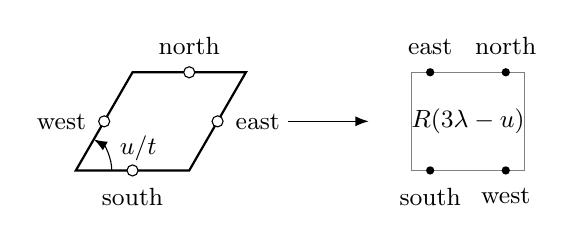
\begin{tikzpicture}[x=1.2cm,y=1.2cm,font=\small,>=Latex]
 \draw[thick] (0,0)--(1.2,0)--(1.8,1.039)--(.6,1.039)--cycle;
 \foreach \x/\y/\label/\pos in {.6/0/south/below,.3/.5195/west/left,1.5/.5195/east/right,1.2/1.039/north/above}{
  \draw[fill=white] (\x,\y) circle (2pt);
  \node[\pos=3pt] at (\x,\y) {\label};
 }
 \draw[->] (.38,0) arc[start angle=0,end angle=60,radius=.38];
 \node at (.66,.23) {$u/t$};
 \draw[->] (2.25,.52)--(3.1,.52);
 \draw[black!50] (3.55,0) rectangle (4.75,1.039);
 \node at (4.15,.52) {$R(3\lambda-u)$};
 \foreach \x/\y/\label/\pos in {3.75/0/south/below,4.55/0/west/below,3.75/1.039/east/above,4.55/1.039/north/above}{
  \fill (\x,\y) circle (1.5pt);
  \node[\pos=3pt] at (\x,\y) {\label};
 }
\end{tikzpicture}
\end{document}
